

\section{backup sides}
\begin{frame}{}
\end{frame}

\begin{frame}{backup slides}
\end{frame}

\subsection{higher-level tools from RMW}
\begin{frame}[fragile]{using atomic exchange?}
    \begin{itemize}
    \item example: OS wants something done by whichever core tries first
    \item does not want it started twice!
    \item if two cores try at once, only one should do it
    \end{itemize}
\begin{lstlisting}[language=C,style=smaller]
int global_flag = 0;
void DoThingIfFirstToTry() {
    int my_value = 1;
    AtomicExchange(&my_value, &global_flag);
    if (my_value == 0) {
        /* flag was zero before, so I was first!*/
        DoThing();
    } else {
        /* flag was already 1 when we exchanged */
        /* I was second, so some other core is handling it */
    }
}
\end{lstlisting}
\end{frame}



\subsection{recall: POSIX mutexes}

\begin{frame}[fragile,label=pthreadMutexBasic]{recall: pthread mutex}
\begin{lstlisting}[language=C++,style=small]
#include <pthread.h>

pthread_mutex_t some_lock;
pthread_mutex_init(&some_lock, NULL);
// or: pthread_mutex_t some_lock = PTHREAD_MUTEX_INITIALIZER;
...
pthread_mutex_lock(&some_lock);
...
pthread_mutex_unlock(&some_lock);
pthread_mutex_destroy(&some_lock);
\end{lstlisting}
\end{frame}



\subsection{even/odd idea for life hw}
\usetikzlibrary{patterns}

\begin{frame}{}
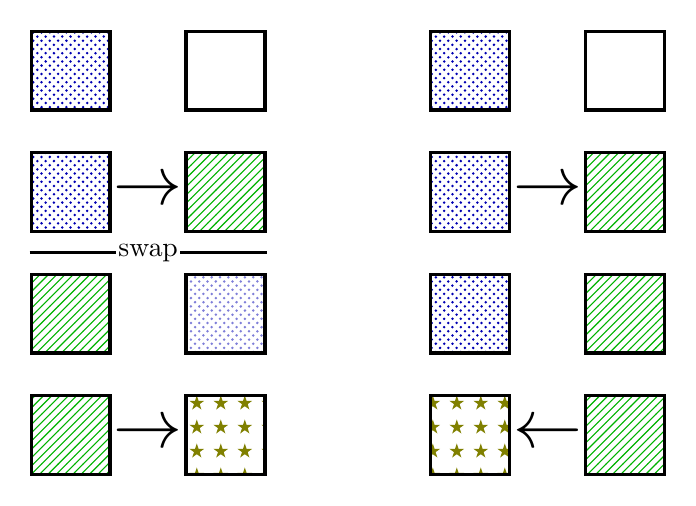
\begin{tikzpicture}
\tikzset{
    grid/.style={anchor=center,draw,very thick,minimum height=1cm,minimum width=1cm},
    grid A/.style={grid,pattern=crosshatch dots,pattern color=blue!70!black},
    grid B/.style={grid,pattern=north east lines,pattern color=green!70!black},
    grid C/.style={grid,pattern=fivepointed stars,pattern color=yellow!50!black},
    faded/.style={fill opacity=0.5},
    for arrow/.style={font=\Huge,anchor=center},
    ampersand replacement=\&,
}
\matrix[row sep=.5cm] (primary) {
    \node[grid A] {}; \& \node[for arrow] {~}; \& \node[grid] (first right) {}; \\
    \node[grid A] (first left) {}; \& \node[for arrow] {$\rightarrow$}; \& \node[grid B] (first right) {}; \\
    \node[grid B] {}; \& \node[for arrow] {~}; \& \node[grid A,faded] {}; \\
    \node[grid B] (second left) {}; \& \node[for arrow] {$\rightarrow$}; \& \node[grid C] (second right) {}; \\
};
    \draw[very thick] ([yshift=-2.5mm]first left.south west) -- ([yshift=-2.5mm]first right.south east)
        node[midway,fill=white]{swap};

\matrix[row sep=.5cm,anchor=north west] (secondary) at ([xshift=2cm]primary.north east) {
    \node[grid A] {}; \& \node[for arrow] {~}; \& \node[grid] {}; \\
    \node[grid A] {}; \& \node[for arrow] {$\rightarrow$}; \& \node[grid B] {}; \\
    \node[grid A] {}; \& \node[for arrow] {~}; \& \node[grid B] {}; \\
    \node[grid C] {}; \& \node[for arrow] {$\leftarrow$}; \& \node[grid B] {}; \\
};
\end{tikzpicture}
\end{frame}


\subsection{x86-64 spinlock}
\begin{frame}[fragile,label=spinlockXchg]{x86-64 spinlock with xchg}
    \begin{itemize}
        \item lock variable in shared memory: \texttt{the\_lock}
        \item if 1: someone has the lock; if 0: lock is free to take
    \end{itemize}
\begin{lstlisting}[
    language=myasm,
    style=smaller,
    morekeywords=mfence,
    moredelim={**[is][\btHL<2|handout:2>]{@2}{2@}},
    moredelim={**[is][\btHL<3|handout:3>]{@3}{3@}},
    moredelim={**[is][\btHL<4|handout:4>]{@4}{4@}},
    moredelim={**[is][\btHL<5|handout:5>]{@5}{5@}},
]
acquire:
    @2movl $1, %eax2@             // %eax <- 1
    @2@5lock5@ xchg %eax, the_lock2@  // swap %eax and the_lock
                                    // sets the_lock to 1 (taken)
                                    // sets %eax to prior val. of the_lock
    @3test %eax, %eax3@           // if the_lock wasn't 0 before:
    @3jne acquire3@               //   try again
    ret

release:
    @5mfence5@                    // for memory order reasons
    @4movl $0, the_lock4@         // then, set the_lock to 0 (not taken)
    ret
\end{lstlisting}
\begin{tikzpicture}[overlay,remember picture]
\coordinate (place) at ([xshift=-1cm,yshift=-1cm]current page.east);
\tikzset{
    box/.style={draw=red,ultra thick,align=left,anchor=east,at={(place)},fill=white},
    box lower/.style={draw=red,ultra thick,align=left,anchor=east,at={(place)},fill=white},
}
\begin{visibleenv}<2>
    \node[box] { set lock variable to 1 (taken) \\ read old value };
\end{visibleenv}
\begin{visibleenv}<3>
    \node[box] { if lock was already locked retry \\ ``spin'' until lock is released elsewhere };
\end{visibleenv}
\begin{visibleenv}<4>
    \node[box] { release lock by setting it to 0 (not taken) \\ allows looping acquire to finish};
\end{visibleenv}
\begin{visibleenv}<5>
    \node[box lower] { Intel's manual says: \\
                 no reordering of loads/stores across a \texttt{lock} \\
                 or \texttt{mfence} instruction
    };
\end{visibleenv}
\end{tikzpicture}
\end{frame}



\subsection{exercise: spin-wait}
\begin{frame}[fragile,label=exerSpinWait]{exercise: spin wait}
\begin{itemize}
\item consider implementing `waiting' functionality of pthread\_join
\vspace{.5cm}
\item thread calls ThreadFinish() when done
\item complete code below:
\end{itemize}
\begin{lstlisting}[language=myasm,style=smaller]
finished: .quad 0
ThreadFinish:
    _________________________
    ret
ThreadWaitForFinish:
    _________________________
    lock xchg %eax, finished
    cmp $0, %eax
    ____ ThreadWaitForFinish
    ret
\end{lstlisting}
\small
\begin{tabular}{lll}
A. \texttt{mfence; mov \$1, finished} & C. \texttt{mov \$0, \%eax} & E. je \\
B. \texttt{mov \$1, finished; mfence} & D. \texttt{mov \$1, \%eax} & F. jne  \\
\end{tabular}
\end{frame}

\begin{frame}<0>[fragile,label=exerSpinWaitSoln]{exercise: spin wait}
\begin{lstlisting}[language=myasm,style=smaller]
finished: .quad 0
ThreadFinish:
    __________A______________
    ret
ThreadWaitForFinish:            /* or without using a writing instruction: */
    _________B______________    mov %eax, finished
    lock xchg %eax, finished    mfence
    cmp $0, %eax                cmp $0, %eax
    __C_ ThreadWaitForFinish    je ThreadWaitForFinish
    ret                         ret
\end{lstlisting}
\small
\begin{tabular}{lll}
A. \texttt{mfence; mov \$1, finished} & C. \texttt{mov \$0, \%eax} & E. je \\
B. \texttt{mov \$1, finished; mfence} & D. \texttt{mov \$1, \%eax} & F. jne  \\
\end{tabular}
\end{frame}
\iftoggle{heldback}{}{\againframe<1>{exerSpinWaitSoln}}


\subsection{spinlock problems}
\begin{frame}<1>[fragile,label=spinLockProblems]{spinlock problems}
    \begin{itemize}
    \item \myemph<4>{lock abstraction is not powerful enough}
        \begin{itemize}
        \item lock/unlock operations don't handle ``wait for event''
        \item common thing we want to do with threads
        \item solution: other synchronization abstractions
        \end{itemize}
    \item \myemph<3>{spinlocks waste CPU time more than needed}
        \begin{itemize}
        \item want to run another thread instead of infinite loop
        \item solution: lock implementation integrated with scheduler
        \end{itemize}
    \item \myemph<2>{spinlocks can send a lot of messages on the shared bus}
        \begin{itemize}
        \item more efficient atomic operations to implement locks
        \end{itemize}
    \end{itemize}
\end{frame}


\subsection{motivation: threaded ATM server?}
\usetikzlibrary{fit}
% 

\begin{frame}{example application: ATM server}
\begin{itemize}
    \item commands: withdraw, deposit
    \item one correctness goal: don't lose money
\end{itemize}
\end{frame}

\begin{frame}[fragile,label=serverCode]{ATM server}
\vspace{-.5cm}
{\small (pseudocode)}
\begin{lstlisting}[language=C++,style=small]
ServerLoop() {
    while (true) {
        ReceiveRequest(&operation, &accountNumber, &amount);
        if (operation == DEPOSIT) {
            Deposit(accountNumber, amount);
        } else ...
    }
}
Deposit(accountNumber, amount) {
    account = GetAccount(accountNumber);
    account->balance += amount;
    SaveAccountUpdates(account);
}
\end{lstlisting}
\end{frame}


\begin{frame}[fragile,label=threadedServerLoop]{multiple threads}
\begin{lstlisting}[
    language=C++,
    style=smaller,
    moredelim={**[is][\btHL<1-|handout:1->]{@1}{1@}}
]
main() {
    for (int i = 0; i < NumberOfThreads; ++i) {
        pthread_create(&server_loop_threads[i], NULL,
                       ServerLoop, NULL);
    }
    ...
}

ServerLoop() {
    while (true) {
        ReceiveRequest(&operation, &accountNumber, &amount);
        if (operation == DEPOSIT) {
            Deposit(accountNumber, amount);
        } else ...
    }
}
\end{lstlisting}
\end{frame}


\subsection{locks that sleep}

\againframe<3>{spinLockProblems}
\begin{frame}{mutexes: intelligent waiting}
\begin{itemize}
    \item want: locks that wait better 
        \begin{itemize}
        \item example: POSIX mutexes
        \end{itemize}
    \item instead of running infinite loop, give away CPU
    \vspace{.5cm}
    \item \myemph<2>{lock = go to sleep}, add self to list
        \begin{itemize}
            \item sleep = scheduler runs something else
        \end{itemize}
    \item \myemph<2>{unlock = wake up sleeping thread}
\end{itemize}
\end{frame}

\begin{frame}{better lock implementation idea}
\begin{itemize}
    \item \textit{shared} list of waiters
    \item \myemph<2>{spinlock protects list of waiters} from concurrent modification
    \vspace{.5cm}
    \item lock = use spinlock to add self to list, then wait without spinlock
    \item unlock = use spinlock to remove item from list
\end{itemize}
\end{frame}



\subsubsection{pseudocode}

\begin{frame}[fragile,label=mutexSketch]{one possible implementation}
\begin{tikzpicture}
\node (header) {
\begin{lstlisting}[
    language=C++,
    style=smaller,
    moredelim={**[is][\btHL<2|handout:2>]{@2}{2@}},
    moredelim={**[is][\btHL<3|handout:3>]{@3}{3@}},
    moredelim={**[is][\btHL<4|handout:4>]{@4}{4@}},
    moredelim={**[is][\btHL<5|handout:5>]{@5}{5@}},
]
struct Mutex { 
    @2SpinLock guard_spinlock;2@
    @3bool lock_taken = false;3@
    @4WaitQueue wait_queue;4@
};
\end{lstlisting}
};
\tikzset{
    box/.style={draw=red,thick,fill=white,font=\small,align=left}
}
\begin{visibleenv}<2>
\node[box,anchor=north west] at ([yshift=-1cm]header.south west) {
    spinlock protecting \texttt{lock\_taken} and \texttt{wait\_queue} \\
    only held for very short amount of time (compared to mutex itself)
};
\end{visibleenv}
\begin{visibleenv}<3>
\node[box,anchor=north west] at ([yshift=-1cm]header.south west) {
    tracks whether any thread has locked and not unlocked
};
\end{visibleenv}
\begin{visibleenv}<4>
\node[box,anchor=north west] at ([yshift=-1cm]header.south west) {
    list of threads that discovered lock is taken \\
    and are waiting for it be free \\
    these threads are \myemph{not runnable}
};
\end{visibleenv}
\begin{visibleenv}<6>
\node[box,anchor=north west] at ([yshift=0cm]header.south west) {
    instead of setting lock\_taken to false \\
    choose thread to hand-off lock to
};
\end{visibleenv}
\begin{visibleenv}<5->
\node[anchor=north west] (lock code) at ([yshift=-1.5cm]header.south west) {
\begin{lstlisting}[
    language=C++,
    basicstyle=\tt\fontsize{8.5}{9.5}\selectfont,
    moredelim={**[is][\btHL<7-8|handout:7-8>]{@6}{6@}},
]
LockMutex(Mutex *m) {
  LockSpinlock(&m->guard_spinlock);
  if (m->lock_taken) {
    put current thread on m->wait_queue
    mark current thread as waiting
    /* xv6: myproc()->state = SLEEPING; */
    @6UnlockSpinlock(&m->guard_spinlock);6@
    @6run scheduler (context switch)6@
  } else {
    m->lock_taken = true;
    UnlockSpinlock(&m->guard_spinlock);
  }
}
\end{lstlisting}
};
\begin{visibleenv}<7>
\node[box,anchor=north west,fill=white] at ([yshift=0cm]header.south west) {
    subtly: if UnlockMutex runs here on another core\\
    need to make sure scheduler on the other core doesn't switch to thread \\
    while it is still running (would `clone' thread/mess up registers)
};
\end{visibleenv}

\node[anchor=north west] (unlock code) at (lock code.north east) {
\begin{lstlisting}[
    language=C++,
    basicstyle=\tt\fontsize{8.5}{9.5}\selectfont,
    moredelim={**[is][\btHL<6|handout:6>]{@5}{5@}},
]
UnlockMutex(Mutex *m) {
  LockSpinlock(&m->guard_spinlock);
  if (m->wait_queue not empty) {
    @5remove a thread from m->wait_queue5@ 
    @5mark thread as no longer waiting5@
    /* xv6: myproc()->state = RUNNABLE; */
  } else {
     m->lock_taken = false;
  }
  UnlockSpinlock(&m->guard_spinlock);
}
\end{lstlisting}
};
\end{visibleenv}
\end{tikzpicture}
\end{frame}



\subsubsection{need for scheduler integration}
\begin{frame}{mutex and scheduler subtly}
\small
\begin{tabular}{l|l|l}
core 0 (thread A) & core 1 (thread B) \\ \hline
    start LockMutex & \\
    acquire spinlock & \\
    discover lock taken & \\
    enqueue thread A & \\
    thread A set not runnable & \\
    release spinlock & start UnlockMutex \\
                 & thread A set runnable  \\
                 & finish UnlockMutex \\
                 & run scheduler \\
                 & scheduler switches to A \\
                 & \myemph<2>{\ldots with old verison of registers} \\
    thread A runs scheduler & & \ldots\\
    \ldots finally saving registers & &\ldots\\
\end{tabular}
\begin{itemize}
\item Linux soln.: track `thread running' separately from `thread runnable'
\item xv6 soln.: hold scheduler lock until thread A saves registers 
\end{itemize}
\end{frame}


\subsubsection{analysis: uncontended case}

\begin{frame}{mutex efficiency}
\begin{itemize}
\item `normal' mutex \textbf{\myemph{uncontended}} case:
    \begin{itemize}
    \item lock: acquire + release spinlock, see lock is free
    \item unlock: acquire + release spinlock, see queue is empty
    \end{itemize}
\vspace{.5cm}
\item not much slower than spinlock
\end{itemize}
\end{frame}



\subsection{disabling interrupts for locks}
\begin{frame}{implementing locks: single core}
    \begin{itemize}
    \item intuition: context switch only happens on interrupt
        \begin{itemize}
        \item timer expiration, I/O, etc. causes OS to run
        \end{itemize}
    \item solution: disable them
        \begin{itemize}
        \item reenable on unlock
        \end{itemize}
    \item<2-> x86 instructions:
        \begin{itemize}
        \item \texttt{cli} --- disable interrupts
        \item \texttt{sti} --- enable interrupts
        \end{itemize}
    \end{itemize}
\end{frame}

\begin{frame}[fragile,label=naiveEnableDisable1]{naive interrupt enable/disable (1)}
\begin{tikzpicture}
\node (lock code) {
\begin{lstlisting}[
    language=C++,
    style=small,
    moredelim={**[is][\color{red}\bfseries]{@1}{1@}},
]    
Lock() {
    @1disable interrupts1@
}
\end{lstlisting}
};
\node[anchor=north west] (unlock code) at ([xshift=1cm]lock code.north east) {
\begin{lstlisting}[
    language=C++,
    style=small,
    moredelim={**[is][\color{red}\bfseries]{@1}{1@}},
]    
Unlock() {
    @1enable interrupts1@
}
\end{lstlisting}
};
\end{tikzpicture}
\begin{itemize}
\item<2-> problem: user can \myemph{hang the system}:
\begin{lstlisting}[
    language=C++,
    style=small,
    moredelim={**[is][\btHL<1-|handout:1->]{@1}{1@}},
]    
            Lock(some_lock);
            while (true) {}
\end{lstlisting}
\item<3-> problem: can't do I/O within lock
\begin{lstlisting}[
    language=C++,
    style=small,
    moredelim={**[is][\btHL<1-|handout:1->]{@1}{1@}},
]    
            Lock(some_lock);
            read from disk
                /* waits forever for (disabled) interrupt
                   from disk IO finishing */
\end{lstlisting}
\end{itemize}
\end{frame}


\begin{frame}[fragile,label=naiveEnableDisable2]{naive interrupt enable/disable (2)}
\begin{tikzpicture}
\node (lock code) {
\begin{lstlisting}[
    language=C++,
    style=small,
    moredelim={**[is][\color{red}\bfseries]{@1}{1@}},
]    
Lock() {
    @1disable interrupts1@
}
\end{lstlisting}
};
\node[anchor=north west] (unlock code) at ([xshift=1cm]lock code.north east) {
\begin{lstlisting}[
    language=C++,
    style=small,
    moredelim={**[is][\color{red}\bfseries]{@1}{1@}},
]    
Unlock() {
    @1enable interrupts1@
}
\end{lstlisting}
};
\end{tikzpicture}
\begin{itemize}
\item<4-> problem: nested locks
\begin{lstlisting}[
    language=C++,
    style=small,
    moredelim={**[is][\color{red}\bfseries]{@1}{1@}},
]    
        Lock(milk_lock);
        if (no milk) {
            Lock(store_lock);
            buy milk
            Unlock(store_lock);
            /* interrupts enabled here?? */
        }
        Unlock(milk_lock);
\end{lstlisting}
\end{itemize}
\end{frame}



%\subsection{xv6's push/popcli}
%\begin{frame}[fragile,label=xv6IntDis1]{xv6 interrupt disabling (1)}
\begin{lstlisting}[
    language=C++,
    style=small,
]
...
acquire(struct spinlock *lk) {
  pushcli(); // disable interrupts to avoid deadlock
  ... /* this part basically just for multicore */
}
release(struct spinlock *lk)
{
  ... /* this part basically just for multicore */
  popcli();
}
\end{lstlisting}
\end{frame}

\begin{frame}{xv6 push/popcli}
\begin{itemize}
\item pushcli / popcli --- need to be in pairs
\item pushcli --- disable interrupts if not already
\item popcli --- enable interrupts if corresponding pushcli disabled them
    \begin{itemize}
    \item don't enable them if they were already disabled
    \end{itemize}
\end{itemize}
\end{frame}


\subsection{aside: standard container rules}
\begin{frame}{C++ containers and locking}
    \begin{itemize}
    \item can you use a vector from multiple threads?
    \item \ldots question: how is it implemented?
        \begin{itemize}
        \item<2-> dynamically allocated array
        \item<2-> reallocated on size changes
        \end{itemize}
    \vspace{.5cm}
    \item<3-> can access from multiple threads \ldots \myemph{as long as not append/erase/etc.}?
    \item<3-> assuming it's implemented like we expect\ldots
        \begin{itemize}
        \item but can we really depend on that?
        \item e.g. could shrink internal array after a while with no expansion save memory?
        \end{itemize}
    \end{itemize}
\end{frame}

\begin{frame}[fragile,label=cppStdRules]{C++ standard rules for containers}
\begin{itemize}
    \item multiple threads can \myemph{read anything at the same time}
    \item can only read element \myemph{if no other thread is modifying it}
    \vspace{.5cm}
    \item can safely \myemph{add/remove elements if no other threads} are accessing container
        \begin{itemize}
            \item (sometimes can safely add/remove in extra cases)
        \end{itemize}
    \vspace{.5cm}
    \item exception: vectors of bools --- can't safely read and write at same time
        \begin{itemize}
        \item might be implemented by putting multiple bools in one int
        \end{itemize}
    \end{itemize}
\end{frame}



\subsection{processor reordering}
\begin{frame}[fragile,label=loadReorderSetup]{a simple race}
\begin{tikzpicture}
\node (thread A code) {
\begin{lstlisting}[language=myasm,style=smaller]
thread_A:
    movl $1, x   /* x <- 1 */
    movl y, %eax /* return y */
    ret
\end{lstlisting}
};
\node[anchor=north west] (thread B code) at ([xshift=.5cm]thread A code.north east) {
\begin{lstlisting}[language=myasm,style=smaller]
thread_B:
    movl $1, y   /* y <- 1 */
    movl x, %eax /* return x */
    ret
\end{lstlisting}
};
\node[anchor=north](driver code) at ([yshift=-.25cm,xshift=-.25cm]thread B code.south west) {
\begin{lstlisting}[language=C++,style=smaller]
x = y = 0;
pthread_create(&A, NULL, thread_A, NULL);
pthread_create(&B, NULL, thread_B, NULL);
pthread_join(A, &A_result); pthread_join(B, &B_result);
printf("A:%d B:%d\n", (int) A_result, (int) B_result);
\end{lstlisting}
};
\end{tikzpicture} 
\begin{itemize}
\item<2-> if loads/stores atomic, then possible results:
    \begin{itemize}
    \item A:1 B:1 --- both moves into x and y, then both moves into eax execute
    \item A:0 B:1 --- thread A executes before thread B
    \item A:1 B:0 --- thread B executes before thread A
    \end{itemize}
\end{itemize}
\end{frame}

\begin{frame}[fragile,label=loadReorderExpResults]{a simple race: results}
\begin{tikzpicture}
\node (thread A code) {
\begin{lstlisting}[language=myasm,style=smaller]
thread_A:
    movl $1, x   /* x <- 1 */
    movl y, %eax /* return y */
    ret
\end{lstlisting}
};
\node[anchor=north west] (thread B code) at ([xshift=.5cm]thread A code.north east) {
\begin{lstlisting}[language=myasm,style=smaller]
thread_B:
    movl $1, y   /* y <- 1 */
    movl x, %eax /* return x */
    ret
\end{lstlisting}
};
\node[anchor=north] (driver code) at ([yshift=-.25cm,xshift=-.25cm]thread B code.south west) {
\begin{lstlisting}[language=C++,style=smaller]
x = y = 0;
pthread_create(&A, NULL, thread_A, NULL);
pthread_create(&B, NULL, thread_B, NULL);
pthread_join(A, &A_result); pthread_join(B, &B_result);
printf("A:%d B:%d\n", (int) A_result, (int) B_result);
\end{lstlisting}
};
\end{tikzpicture} 
\begin{center}
\small my desktop, 100M trials: \\
\begin{tabular}{r|l|l}
frequency & result & ~ \\ \hline
$99\,823\,739$ & A:0 B:1 & (`A executes before B') \\
$171\,161$& A:1 B:0 & (`B executes before A') \\
$4\,706$ & A:1 B:1 & (`execute moves into x+y first') \\
\myemph<2>{$394$} & \myemph<2>{A:0 B:0} & \myemph<2>{???} \\
\end{tabular}
\end{center}
\end{frame}


\subsection{why reorder?}

\begin{frame}[fragile]{why reorder here?}
\begin{tikzpicture}
\node (thread A code) {
\begin{lstlisting}[language=myasm,style=smaller]
thread_A:
    movl $1, x   /* x <- 1 */
    movl y, %eax /* return y */
    ret
\end{lstlisting}
};
\node[anchor=north west] (thread B code) at ([xshift=.5cm]thread A code.north east) {
\begin{lstlisting}[language=myasm,style=smaller]
thread_B:
    movl $1, y   /* y <- 1 */
    movl x, %eax /* return x */
    ret
\end{lstlisting}
};
\end{tikzpicture}
\begin{itemize}
\item thread A: faster to load \texttt{y} right now!
\item \ldots rather than wait for write of \texttt{x} to finish
\end{itemize}
\end{frame}


\usetikzlibrary{calc}

\begin{frame}{load/store reordering}
\begin{itemize}
    \item load/stores atomic, but run \textit{out of order}
    \vspace{.5cm}
    \item recall?: out-of-order processors
    \item processor optimization: sometimes execute instructions in non-program order
        \begin{itemize}
        \item hide delays from slow caches, variable computation rates, etc.
        \item documneted limits on when this is/is not allowed
        \end{itemize}
    \item track side-effects \textit{within a thread} to make as if in-order
        \begin{itemize}
        \item but common choice: don't worry as much between cores/threads
        \item design decision: if programmer cares, they worry about it
        \end{itemize}
    \item want to avoid this \textit{special instructions ensure strict ordering}
\end{itemize}
\end{frame}

\begin{frame}{why load/store reordering?}
\begin{itemize}
\item prior example: load of x executing before store of y
\item why do this? otherwise delay the load
    \begin{itemize}
    \item if x and y unrelated --- no benefit to waiting
    \end{itemize}
\end{itemize}
\end{frame}



\subsection{GCC atomic/sync stuff}
\begin{frame}[fragile,label=prevReorder2]{GCC: preventing reordering example (1)}
\begin{lstlisting}[language=C++,style=smaller]
void Alice() {
    int one = 1;
    __atomic_store(&note_from_alice, &one, __ATOMIC_SEQ_CST);
    do {
    } while (__atomic_load_n(&note_from_bob, __ATOMIC_SEQ_CST));
    if (no_milk) {++milk;}
}
\end{lstlisting}
\hrule
\begin{lstlisting}[language=myasm,style=small,morekeywords=mfence]
Alice:
  movl $1, note_from_alice
  mfence
.L2:
  movl note_from_bob, %eax
  testl %eax, %eax
  jne .L2
  ...
\end{lstlisting}
\end{frame}

\begin{frame}[fragile,label=prevReorder1]{GCC: preventing reordering example (2)}
\begin{lstlisting}[language=C++,style=small]
void Alice() {
    note_from_alice = 1;
    do {
        __atomic_thread_fence(__ATOMIC_SEQ_CST);
    } while (note_from_bob);
    if (no_milk) {++milk;}
}
\end{lstlisting}
\hrule
\begin{lstlisting}[language=myasm,style=small,morekeywords=mfence]
Alice:
  movl $1, note_from_alice  // note_from_alice <- 1
.L3:
  mfence  // make sure store is visible to other cores before loading
          // on x86: not needed on second+ iteration of loop
  cmpl $0, note_from_bob  // if (note_from_bob == 0) repeat fence
  jne .L3
  cmpl $0, no_milk
  ...
\end{lstlisting}
\end{frame}




\subsection{exercise: atomic add}
\begin{frame}[fragile,label=atomicOpEx]{exercise: fetch-and-add with compare-and-swap}
\begin{itemize}
\item exercise: implement fetch-and-add with compare-and-swap
\end{itemize}
\begin{lstlisting}[language=C++,style=smaller,deletekeywords=register]
compare_and_swap(address, old_value, new_value) {
    if (memory[address] == old_value) {
        memory[address] = new_value;
        return true;   // x86: set ZF flag
    } else {
        return false;  // x86: clear ZF flag
    }
}
\end{lstlisting}
\end{frame}

\iftoggle{heldback}{
    \excludecomment{heldbackstuff}
}{
    \includecomment{heldbackstuff}
}

\begin{frame}[fragile,label=atomicAdd]{solution}
\begin{heldbackstuff}
\begin{lstlisting}[language=C++,style=smaller,deletekeywords=register]
long my_fetch_and_add(long *p, long amount) {
    long old_value;
    do {
        old_value = *p;
    while (!compare_and_swap(p, old_value, old_value + amount);
    return old_value;
}
\end{lstlisting}
\end{heldbackstuff}
\end{frame}

\subsection{xv6's spinlock debugging}

\begin{frame}[fragile,label=xv6SpinlockAcquire]{xv6 spinlock: acquire}
\begin{lstlisting}[
    language=C++,
    style=smaller,
    morekeywords=mfence,
    moredelim={**[is][\btHL<2|handout:2>]{@2}{2@}},
    moredelim={**[is][\btHL<3|handout:3>]{@3}{3@}},
    moredelim={**[is][\btHL<4|handout:4>]{@4}{4@}},
    moredelim={**[is][\btHL<5|handout:5>]{@5}{5@}},
]
void
acquire(struct spinlock *lk)
{
  @2pushcli();2@ // disable interrupts to avoid deadlock.
  ...
  // The xchg is atomic.
  @3while(xchg(&lk->locked, 1) != 0)3@
    ; 

  // Tell the C compiler and the processor to not move loads or stores
  // past this point, to ensure that the critical section's memory
  // references happen after the lock is acquired.
  @4__sync_synchronize();4@
  ...
}
\end{lstlisting}
\begin{tikzpicture}[overlay,remember picture]
\coordinate (place) at ([yshift=1cm]current page.south);
\coordinate (place higher) at ([yshift=3cm]current page.south);
\tikzset{
    box/.style={draw=red,ultra thick,fill=white,align=left,at={(place)},anchor=south},
    box higher/.style={draw=red,ultra thick,fill=white,align=left,at={(place higher)},anchor=south},
}
\begin{visibleenv}<2>
    \node[box] {
        don't let us be interrupted after while have the lock \\
        problem: interruption might try to do something with the lock \\
        \ldots but that can never succeed until we release the lock \\
        \ldots but we won't release the lock until interruption finishes
    };
\end{visibleenv}
\begin{visibleenv}<3>
    \node[box] {
        xchg wraps the lock xchg instruction \\
        same loop as before
    };
\end{visibleenv}
\begin{visibleenv}<4>
    \node[box] {
        avoid load store reordering (including by compiler) \\
        on x86, \texttt{xchg} alone is enough to avoid processor's reordering \\
        (but compiler may need more hints)
    };
\end{visibleenv}
\end{tikzpicture}
\end{frame}

\begin{frame}[fragile,label=xv6SpinlockRelease]{xv6 spinlock: release}
\begin{lstlisting}[
    language=C++,
    style=smaller,
    morekeywords=mfence,
    moredelim={**[is][\btHL<2|handout:2>]{@2}{2@}},
    moredelim={**[is][\btHL<3|handout:3>]{@3}{3@}},
    moredelim={**[is][\btHL<4|handout:4>]{@4}{4@}},
    moredelim={**[is][\btHL<5|handout:5>]{@5}{5@}},
]
void
release(struct spinlock *lk)
  ...
  // Tell the C compiler and the processor to not move loads or stores
  // past this point, to ensure that all the stores in the critical
  // section are visible to other cores before the lock is released.
  // Both the C compiler and the hardware may re-order loads and
  // stores; __sync_synchronize() tells them both not to.
  @2__sync_synchronize();2@

  // Release the lock, equivalent to lk->locked = 0.
  // This code can't use a C assignment, since it might
  // not be atomic. A real OS would use C atomics here.
  @3asm volatile("movl $0, %0" : "+m" (lk->locked) : );3@

  @4popcli();4@
}
\end{lstlisting}
\begin{tikzpicture}[overlay,remember picture]
\coordinate (place) at ([yshift=1cm]current page.south);
\tikzset{
    box/.style={draw=red,ultra thick,fill=white,align=left,at={(place)},anchor=south},
}
\begin{visibleenv}<2>
    \node[box] {
        turns into instruction to tell processor not to reorder \\
        plus tells compiler not to reorder
    };
\end{visibleenv}
\begin{visibleenv}<3>
    \node[box] {
        turns into mov of constant 0 into \lstinline|lk->locked|
    };
\end{visibleenv}
\begin{visibleenv}<4>
    \node[box] {
        reenable interrupts (taking nested locks into account)
    };
\end{visibleenv}
\end{tikzpicture}
\end{frame}


\subsection{CAS for fetch-and-add}
\begin{frame}[fragile,label=fetchAndAddWithCASSetup]{fetch-and-add with CAS (1)}
\begin{lstlisting}[language=C++,style=smaller,deletekeywords=register]
compare-and-swap(address, old_value, new_value) {
    if (memory[address] == old_value) {
        memory[address] = new_value;
        return true;
    } else {
        return false;
    }
}
\end{lstlisting}
\hrule
\begin{lstlisting}[language=C++,style=smaller,deletekeywords=register]
long my_fetch_and_add(long *pointer, long amount) { ... }
\end{lstlisting}
    \begin{itemize}
    \item implementation sketch:
        \begin{itemize}
        \item fetch value from pointer \texttt{old}
        \item compute in temporary value result of addition \texttt{new}
        \item try to change value at pointer from \texttt{old} to \texttt{new} [\texttt{compare-and-swap}]
        \item if not successful, repeat
        \end{itemize}
    \end{itemize}
\end{frame}

\begin{frame}[fragile,label=fetchAndAddWithCASSoln]{fetch-and-add with CAS (2)}
\begin{lstlisting}[language=C++,style=smaller,deletekeywords=register]
long my_fetch_and_add(long *p, long amount) {
    long old_value;
    do {
        old_value = *p;
    } while (!compare_and_swap(p, old_value, old_value + amount);
    return old_value;
}
\end{lstlisting}
\end{frame}



\subsection{exercise: CAS for appending to list}
\begin{frame}[fragile,label=appendToListExercise]{exercise: append to singly-linked list}
\begin{itemize}
    \item ListNode is a singly-linked list
    \item assume: threads \textit{only} append to list (no deletions, reordering)
    \item use \texttt{compare-and-swap(pointer, old, new)}:
        \begin{itemize}
        \item atomically change \texttt{*pointer} from \texttt{old} to \texttt{new}
        \item return true if successful
        \item return false (and change nothing) if \texttt{*pointer} is not \texttt{old}
        \end{itemize}
\end{itemize}
\begin{lstlisting}[language=C++,style=smaller]
void append_to_list(ListNode *head, ListNode *new_last_node) {
    ...
}
\end{lstlisting}
\end{frame}

\begin{frame}<0>[fragile,label=appendToListSol]{append to singly-linked list}
\begin{lstlisting}[language=C++,style=smaller]
/* assumption: other threads may be appending to list,
 *             but nodes are not being removed, reordered, etc.
 */
void append_to_list(ListNode *head, ListNode *new_last_node) {
  memory_ordering_fence();
  ListNode *current_last_node;
  do {
    current_last_node = head;
    while (current_last_node->next) {
      current_last_node = current_last_node->next;
    }
  } while (
    !compare-and-swap(&current_last_node->next,
                      NULL, new_last_node)
  );
}
\end{lstlisting}
\end{frame}

\iftoggle{heldback}{}{\againframe<1>{appendToListSol}}


\subsection{more atomic operations}


\begin{frame}[fragile,label=moreCommonAtomic1]{some common atomic operations (1)}
\begin{lstlisting}[language=C++,style=smaller,deletekeywords=register]
// x86: emulate with exchange
test_and_set(address) {
    old_value = memory[address];
    memory[address] = 1;
    return old_value != 0;  // e.g. set ZF flag
}

// x86: xchg REGISTER, (ADDRESS)
exchange(register, address) {
    temp = memory[address];
    memory[address] = register;
    register = temp;
}
\end{lstlisting}
\end{frame}

\begin{frame}[fragile,label=moreCommonAtomic2]{some common atomic operations (2)}
\begin{lstlisting}[language=C++,style=smaller,deletekeywords=register]
// x86: mov OLD_VALUE, %eax; lock cmpxchg NEW_VALUE, (ADDRESS)
compare-and-swap(address, old_value, new_value) {
    if (memory[address] == old_value) {
        memory[address] = new_value;
        return true;   // x86: set ZF flag
    } else {
        return false;  // x86: clear ZF flag
    }
}

// x86: lock xaddl REGISTER, (ADDRESS)
fetch-and-add(address, register) {
    old_value = memory[address];
    memory[address] += register;
    register = old_value;
}
\end{lstlisting}
\end{frame}

\begin{frame}{common atomic operation pattern}
    \begin{itemize}
    \item try to do operation, \ldots
    \item detect if it failed
    \item if so, repeat
    \vspace{.5cm}
    \item atomic operation does ``try and see if it failed'' part
    \end{itemize}
\end{frame}





\subsection{cache coherency detail}
\subsection{adding more state: MSI}
\usetikzlibrary{arrows.meta,matrix,positioning,shapes.callouts}

\begin{frame}{cache coherency states}
\begin{itemize}
\item extra information for \myemph{each cache block}
    \begin{itemize}
        \item overlaps with/replaces valid, dirty bits
    \end{itemize}
\item stored in \myemph{each cache}
\item update states based on reads, writes \myemph{and heard messages on bus}
\item different caches may have different states for same block
\end{itemize}
\end{frame}

\begin{frame}{MSI state summary}
\begin{tabular}{lp{10cm}}
{\bfseries Modified} & {value may be \myemph{different than memory} \textit{and} I am the only one who has it } \\
~ & ~ \\
{\bfseries Shared} & value is the \myemph{same as memory} \\
~ & ~ \\
{\bfseries Invalid} & I don't have the value; I will need to ask for it \\
\end{tabular}
\end{frame}

\begin{frame}{MSI scheme}
\begin{tabular}{lllll}
from state & hear read & hear write & read & write \\ \hline
Invalid & --- & --- & \color{blue}to Shared & \color{blue}to Modified \\
Shared & --- & to Invalid & --- & \color{blue}to Modified \\
Modified & \color{blue}to Shared & \color{blue}to Invalid & --- & --- \\
\end{tabular}
\begin{itemize}
\item {\color{blue}blue}: transition requires sending message on bus
\item<2-> example: write while Shared 
    \begin{itemize}
    \item must send write --- inform others with Shared state
    \item then change to Modified
    \end{itemize}
\item<3-> example: hear write while Shared
    \begin{itemize}
    \item change to Invalid
    \item can send read later to get value from writer
    \end{itemize}
\item<3-> example: write while Modified
    \begin{itemize}
    \item nothing to do --- no other CPU can have a copy
    \end{itemize}
\end{itemize}
\end{frame}

\begin{frame}[fragile,label=msiExample]{MSI example}
\begin{tikzpicture}
\matrix[
    matrix of nodes,
    nodes in empty cells,
    row 1/.style={nodes={minimum height=1cm,minimum width=1cm}},
    row 2/.style={nodes={draw,rectangle,minimum height=1cm,minimum width=1cm}},
    column sep=2.75cm,
] (net) {
      \& \& \\
    CPU1 \& CPU2 \& MEM1 \\
};
\foreach \x in {1,2,3} {
    \draw[thick] (net-2-\x.north) -- (net-1-\x.center);
}
\draw[thick,Latex-Latex] (net-1-1.west) -- (net-1-3.east);
\tikzset{
    cache/.style={
        tight matrix,
        nodes={font=\small\ttfamily,text width=1.8cm,execute at begin node={\strut}},
        row 1/.append style={nodes={font=\small\bfseries}},
        column 3/.append style={nodes={font=\sffamily\small}},
    },
}
\matrix[cache,anchor=north] (cache1) at (net-2-1.south east){
    address \& value \& state\\
    0xA300 \& \only<1-2>{\sout<2->{100}}\only<2-3>{\sout<3->{\myemph<2>{101}}}\only<3->{\myemph<3,5>{102}} 
           \& \only<1>{Shared}\only<2-4>{\myemph<2>{Modified}}\only<5->{\myemph<5>{Shared}}\\
    0xC400 \& 200 \& Shared\\
    0xE500 \& 300 \& Shared \\
};
\matrix[cache,anchor=north] (cache2) at ([xshift=1.5cm]net-2-2.south east){
    address \& value \& state\\
    0x9300 \& 172 \& Shared \\ 
    \sout<2->{0xA300} \& \sout<2->{100}\only<6->{\myemph<6>{102}} \& \only<1>{Shared}\only<2-5>{\myemph<2>{Invalid}}\only<6>{\myemph<6>{Shared}} \\
    0xC500 \& 200 \& Shared\\
};
\begin{visibleenv}<2>
    \draw[blue,very thick,-Latex]  (net-2-1.north) -- (net-1-1.center) 
        node[above,xshift=2cm] {``CPU1 is writing 0xA3000''} -- (net-1-2.center) --(net-2-2.north);
    \draw[blue,dashed,very thick,-Latex]  (net-2-1.north) -- (net-1-1.center) -- (net-1-3.center) --(net-2-3.north);
\node[draw,thick,draw=blue,rectangle,anchor=north west] at ([yshift=-1cm]cache1.south west){
    CPU1 writes 101 to 0xA300
};
\node[my callout2=cache2-3-2,anchor=north,align=left] at ([yshift=-.5cm]cache2-3-2.south) {
    cache sees write: \\ invalidate 0xA300
};
\node[my callout2=net-2-3.center,anchor=south] at ([yshift=1.5cm,xshift=-1.5cm]net-2-3.center) {
    maybe update memory?
};
\end{visibleenv}
\begin{visibleenv}<3>
\node[draw,thick,draw=blue,rectangle,anchor=north west] (writeTo) at ([yshift=-1cm]cache1.south west){
    CPU1 writes 102 to 0xA300
};
\node[my callout2=cache1-2-3,anchor=north,align=left] at ([xshift=2cm,yshift=-.5cm]cache1-2-2.south) {
    modified state --- nothing communicated! \\
    will ``fix'' later if there's a read
};
\node[my callout2=net-2-3.center,anchor=south] at ([yshift=1.5cm,xshift=-2cm]net-2-3.center) {
    nothing changed yet (\myemph{writeback})
};
\end{visibleenv}
\begin{visibleenv}<4>
    \draw[blue,dashed,very thick,-Latex]  (net-2-2.north) -- (net-1-2.center) -- (net-1-1.center) --(net-2-1.north);
    \draw[blue,very thick,-Latex]  (net-2-2.north) -- (net-1-2.center) node[above] {``What is 0xA300?''} -- (net-1-3.center) --(net-2-3.north);
\node[draw,thick,draw=blue,rectangle,anchor=north west] at ([yshift=-1cm]cache2.south west){
    CPU2 reads 0xA300
};
\node[my callout2=cache1-2-2,anchor=north] at ([yshift=-.5cm]cache1-2-3.south) {
    modified state --- must update for CPU2!
};
\end{visibleenv}
\begin{visibleenv}<5>
    \draw[blue,dashed,very thick,-Latex]  (net-2-1.north) -- (net-1-1.center) -- (net-1-3.center) --(net-2-3.north);
    \draw[blue,very thick,-Latex]  (net-2-1.north) -- (net-1-1.center) node[above,xshift=1cm] {``Write 102 into 0xA300''} -- (net-1-3.center) --(net-2-3.north);
\node[draw,thick,draw=blue,rectangle,anchor=north west] at ([yshift=-1cm]cache2.south west){
    CPU2 reads 0xA300
};
\node[my callout2=cache1-2-2,anchor=north,align=left] at ([yshift=-.5cm]cache1-2-3.south) {
    written back to memory early \\
    (could also become Invalid at CPU1)
};
\end{visibleenv}
\end{tikzpicture}
\end{frame}

\begin{frame}{MSI: update memory}
\begin{itemize}
    \item to write value (enter modified state), need to \myemph{invalidate} others
    \item can avoid sending actual value (shorter message/faster)
    \vspace{.5cm}
    \item ``I am writing address $X$'' versus ``I am writing $Y$ to address $X$''
\end{itemize}
\end{frame}

\begin{frame}{MSI: on cache replacement/writeback}
\begin{itemize}
    \item still happens --- e.g. want to store something else
    \item changes state to \myemph{invalid}
    \item requires writeback if modified (= dirty bit)
\end{itemize}
\end{frame}




\subsection{exercise}
\begin{frame}{cache coherency exercise}
\begin{itemize}
\item modified/shared/invalid; all initially invalid; 32B blocks, 8B read/writes
\begin{itemize}
\item CPU 1: read 0x1000
\item CPU 2: read 0x1000
\item CPU 1: write 0x1000
\item CPU 1: read 0x2000
\item CPU 2: read 0x1000
\item CPU 2: write 0x2008
\item CPU 3: read 0x1008
\end{itemize}
\item Q1: final state of 0x1000 in caches? 
    \begin{itemize}
    \item Modified/Shared/Invalid for CPU 1/2/3
    \item CPU 1: \hspace{2cm} CPU 2: \hspace{2cm} CPU 3: \hspace{2cm}
    \end{itemize}
\item Q2: final state of 0x2000 in caches? 
    \begin{itemize}
    \item Modified/Shared/Invalid for CPU 1/2/3
    \item CPU 1: \hspace{2cm} CPU 2: \hspace{2cm} CPU 3: \hspace{2cm}
    \end{itemize}
\end{itemize}
\end{frame}

\begin{frame}<0>[label=cacheCoherenceExSoln]{cache coherency exercise solution}
\tt
\begin{tabular}{l|ccc|ccc}
~ & \multicolumn{3}{c|}{\tt 0x1000-0x101f} & \multicolumn{3}{c}{\tt 0x2000-0x201f} \\
\normalfont\bfseries action & \normalfont CPU 1 & \normalfont CPU 2 & \normalfont CPU 3 & \normalfont CPU 1 & \normalfont CPU 2 & \normalfont CPU 3 \\ \hline
~   & I & I & I & I & I & I \\
\normalfont CPU 1: read \tt 0x1000
    & \myemph{S} & I & I & I & I & I \\
\normalfont CPU 2: read \tt 0x1000
    & S & \myemph{S} & I & I & I & I \\
\normalfont CPU 1: write \tt 0x1000
    & \myemph{M} & \myemph{I} & I & I & I & I \\
\normalfont CPU 1: read \tt 0x2000
    & M & I & I & \myemph{S} & I & I \\
\normalfont CPU 2: read \tt 0x1000 
    & \myemph{S} & \myemph{S} & I & S & I & I \\
\normalfont CPU 2: write \tt 0x2008
    & S & S & I & \myemph{I} & \myemph{M} & I \\
\normalfont CPU 3: read \tt 0x1008
    & S & S & \myemph{S} & I & M & I \\
\end{tabular}
%\item CPU 1: read 0x1000
%\item CPU 2: read 0x1000
%\item CPU 1: write 0x1000
%\item CPU 1: read 0x2000
%\item CPU 2: read 0x1000
%\item CPU 2: write 0x2008
%\item CPU 3: read 0x1008
\end{frame}

\iftoggle{heldback}{}{
    \againframe<1->{cacheCoherenceExSoln}
}


\section{processor load/store reordering}
% FIXME: instruction queue/etc. picture?
\usetikzlibrary{calc}

\begin{frame}{load/store reordering}
\begin{itemize}
    \item load/stores atomic, but run \textit{out of order}
    \vspace{.5cm}
    \item recall?: out-of-order processors
    \item processor optimization: sometimes execute instructions in non-program order
        \begin{itemize}
        \item hide delays from slow caches, variable computation rates, etc.
        \item documneted limits on when this is/is not allowed
        \end{itemize}
    \item track side-effects \textit{within a thread} to make as if in-order
        \begin{itemize}
        \item but common choice: don't worry as much between cores/threads
        \item design decision: if programmer cares, they worry about it
        \end{itemize}
    \item want to avoid this \textit{special instructions ensure strict ordering}
\end{itemize}
\end{frame}

\begin{frame}{why load/store reordering?}
\begin{itemize}
\item prior example: load of x executing before store of y
\item why do this? otherwise delay the load
    \begin{itemize}
    \item if x and y unrelated --- no benefit to waiting
    \end{itemize}
\end{itemize}
\end{frame}



\subsection{C++atomic/sync stuff}


\begin{frame}{C++: preventing reordering}
    \begin{itemize}
        \item to help \myemph{implementing things like pthread\_mutex\_lock}
        \vspace{.5cm}
    \item C++ 2011 standard: \textit{atomic} header, \textit{std::atomic} class
        \item prevent CPU reordering \textit{and} prevent compiler reordering
        \item also provide other tools for implementing locks (more later)
            \vspace{.5cm}
        \item could also hand-write assembly code
            \begin{itemize}
                \item compiler can't know what assembly code is doing
            \end{itemize}
    \end{itemize}
\end{frame}

\begin{frame}[fragile,label=prevReorderCpp1]{C++: preventing reordering example}
\begin{lstlisting}[language=C++,style=smaller]
#include <atomic>
void Alice() {
    note_from_alice = 1;
    do {
        std::atomic_thread_fence(std::memory_order_seq_cst);
    } while (note_from_bob);
    if (no_milk) {++milk;}
}
\end{lstlisting}
\hrule
\begin{lstlisting}[language=myasm,style=smaller,morekeywords=mfence]
Alice:
  movl $1, note_from_alice  // note_from_alice <- 1
.L2:
  mfence  // make sure store visible on/from other cores
  cmpl $0, note_from_bob  // if (note_from_bob == 0) repeat fence
  jne .L2
  cmpl $0, no_milk
  ...
\end{lstlisting}
\end{frame}

\begin{frame}[fragile,label=prevReorderCpp2]{C++ atomics: no reordering}
\begin{lstlisting}[language=C++,style=smaller]
std::atomic<int> note_from_alice, note_from_bob;
void Alice() {
    note_from_alice.store(1);
    do {
    } while (note_from_bob.load());
    if (no_milk) {++milk;}
}
\end{lstlisting}
\hrule
\begin{lstlisting}[language=myasm,style=small,morekeywords=mfence]
Alice:
  movl $1, note_from_alice
  mfence
.L2:
  movl note_from_bob, %eax
  testl %eax, %eax
  jne .L2
  ...
\end{lstlisting}
\end{frame}
\begin{frame}{GCC: built-in atomic functions}
    \begin{itemize}
    \item used to implement std::atomic, etc.
    \item predate std::atomic
        \vspace{.5cm}
    \item builtin functions starting with \texttt{\_\_sync} and \texttt{\_\_atomic}
    \item these are what xv6 uses
    \end{itemize}
\end{frame}



\subsection{x86-64 reordering rules}

\begin{frame}{aside: some x86 reordering rules}
\begin{itemize}
\item each core sees its own loads/stores in order
    \begin{itemize}
    \item (if a core stores something, it can always load it back)
    \end{itemize}
\item stores \textit{from other cores} appear in a consistent order
    \begin{itemize}
    \item (but a core might observe its own stores too early)
    \end{itemize}
\item \textit{causality}: \\
    \textit{if} a core reads X=a and (after reading X=a) writes Y=b, \\
    \textit{then} a core that reads Y=b cannot later read X=older value than a
\end{itemize}
\imagecredit{Source: Intel 64 and IA-32 Software Developer's Manual, Volume 3A, Chapter 8}
\end{frame}

\begin{frame}{how do you do anything with this?}
    \begin{itemize}
    \item difficult to reason about what modern CPU's reordering rules do
    \item typically: don't depend on details, instead:
    \vspace{.5cm}
    \item special instructions with stronger (and simpler) ordering rules
        \begin{itemize}
        \item often same instructions that help with implementing locks in other ways
        \end{itemize}
    \item special instructions that restrict ordering of instructions around them (``fences'')
        \begin{itemize}
        \item loads/stores can't cross the fence
        \end{itemize}
    \end{itemize}
\end{frame}




\subsection{test-and-test-and-set}

\againframe<2>{spinLockProblems}
% FIXME: what 3 CPUs, ping-pong between CPU2 and CPU3
\usetikzlibrary{arrows.meta,matrix,positioning,shapes.callouts}

\begin{frame}{ping-ponging}
\begin{tikzpicture}
\matrix[
    matrix of nodes,
    nodes in empty cells,
    row 1/.style={nodes={minimum height=1cm,minimum width=1cm}},
    row 2/.style={nodes={draw,rectangle,minimum height=1cm,minimum width=1cm}},
    column sep=2.75cm,
] (net) {
    \& \& \& \\
    CPU1 \& CPU2 \& CPU3 \& MEM1 \\
};
\foreach \x in {1,2,3,4} {
    \draw[thick] (net-2-\x.north) -- (net-1-\x.center);
}
\draw[thick,Latex-Latex] (net-1-1.west) -- (net-1-4.east);
\tikzset{
    cache/.style={
        tight matrix,
        nodes={font=\fontsize{9}{10}\ttfamily\selectfont,text width=1.5cm,execute at begin node={\strut}},
        row 1/.append style={nodes={font=\fontsize{9}{10}\bfseries\selectfont}},
        column 3/.append style={nodes={font=\fontsize{9}{10}\sffamily\selectfont}},
    },
}
\matrix[cache,anchor=north] (cache1) at (net-2-1.south east){
    address \& value \& state\\
    lock \& \only<1>{locked}\only<2-5,7>{\myemph<2,7>{---}}\only<6>{\myemph<6>{unlocked}} \& \only<1,6>{Modified}\only<2-5,7>{\myemph{Invalid}} \\
};
\matrix[cache,anchor=north] (cache2) at ([xshift=.75cm]net-2-2.south east){
    address \& value \& state\\
    lock \& \only<1,3,5-6>{---}\only<2,4,7>{\myemph{locked}} \& \only<1,3,5,6>{\myemph<2,4>{Invalid}}\only<2,4,7>{\myemph{Modified}} \\
};
\matrix[cache,anchor=north] (cache3) at ([xshift=1.5cm]net-2-3.south east){
    address \& value \& state\\
    lock \& \only<1-2,4>{---}\only<3,5>{\myemph{locked}} \& \only<1-2,4,6-7>{\myemph<4>{Invalid}}\only<3,5>{\myemph{Modified}} \\
};
\begin{visibleenv}<2,4>
    \draw[blue,dashed,very thick,-Latex]  (net-2-2.north) -- (net-1-2.center) -- (net-1-1.center) --(net-2-1.north);
    \draw[blue,very thick,-Latex]  (net-2-2.north) -- (net-1-2.center) node[above] {``I want to modify \texttt{lock}?''} -- (net-1-4.center) --(net-2-4.north);
\node[align=center,draw,thick,draw=blue,rectangle,anchor=north west] at ([yshift=-1cm]cache1.south west){
    CPU2 read-modify-writes lock \\ (to see it is still locked)
};
\end{visibleenv}
\begin{visibleenv}<3,5>
    \draw[blue,dashed,very thick,-Latex]  (net-2-3.north) -- (net-1-3.center) -- (net-1-4.center) --(net-2-4.north);
    \draw[blue,very thick,-Latex]  (net-2-3.north) -- (net-1-3.center) node[above,xshift=1cm] {``I want to modify \texttt{lock}''} -- (net-1-2.center) --(net-2-2.north);
\node[align=center,draw,thick,draw=blue,rectangle,anchor=north west] at ([yshift=-1cm]cache1.south west){
    CPU3 read-modify-writes lock \\ (to see it is still locked)
};
\end{visibleenv}
\begin{visibleenv}<6>
    \draw[blue,dashed,very thick,-Latex]  (net-2-1.north) -- (net-1-1.center) -- (net-1-4.center) --(net-2-4.north);
    \draw[blue,very thick,-Latex]  (net-2-1.north) -- (net-1-1.center) node[above,xshift=1cm] {``I want to modify \texttt{lock}''} -- (net-1-3.center) --(net-2-3.north);
\node[align=center,draw,thick,draw=blue,rectangle,anchor=north west] at ([yshift=-1cm]cache1.south west){
    CPU1 sets lock to unlocked
};
\end{visibleenv}
\begin{visibleenv}<7>
    \draw[blue,dashed,very thick,-Latex]  (net-2-1.north) -- (net-1-1.center) -- (net-1-4.center) --(net-2-4.north);
    \draw[blue,very thick,-Latex]  (net-2-1.north) -- (net-1-1.center) node[above,xshift=1cm] {``I want to modify \texttt{lock}''} -- (net-1-3.center) --(net-2-3.north);
\node[align=center,draw,thick,draw=blue,rectangle,anchor=north west] at ([yshift=-1cm]cache1.south west){
    some CPU (this example: CPU2) acquires lock
};
\end{visibleenv}
\end{tikzpicture}
\end{frame}

\begin{frame}{ping-ponging}
    \begin{itemize}
    \item test-and-set problem: cache block ``ping-pongs'' between caches
        \begin{itemize}
        \item each waiting processor reserves block to modify
        \item could maybe wait until it determines modification needed --- but not typical implementation
        \end{itemize}
    \item each transfer of block sends messages on bus
    \item \ldots so bus can't be used for real work
        \begin{itemize}
        \item like what the processor with the lock is doing
        \end{itemize}
    \end{itemize}
\end{frame}

\begin{frame}[fragile,label=testAndTestAndSetC]{test-and-test-and-set (pseudo-C)}
\begin{lstlisting}[language=C,style=smaller]
acquire(int *the_lock) {
    do {
        while (ATOMIC-READ(the_lock) == 0) { /* try again */ }
    } while (ATOMIC-TEST-AND-SET(the_lock) == ALREADY_SET);
}
\end{lstlisting}
\end{frame}

\begin{frame}[fragile,label=testAndTestAndSetASM]{test-and-test-and-set (assembly)}
\begin{lstlisting}[language=myasm,style=smaller]
acquire:
    cmp $0, the_lock         // test the lock non-atomically
            // unlike lock xchg --- keeps lock in Shared state!
    jne acquire              // try again (still locked)
    // lock possibly free
    // but another processor might lock
    // before we get a chance to
    // ... so try wtih atomic swap:
    movl $1, %eax             // %eax <- 1
    lock xchg %eax, the_lock  // swap %eax and the_lock
           // sets the_lock to 1
           // sets %eax to prior value of the_lock
    test %eax, %eax           // if the_lock wasn't 0 (someone else got it first):
    jne acquire               //   try again
    ret
\end{lstlisting}
\end{frame}

\begin{frame}{less ping-ponging}
\begin{tikzpicture}
\matrix[
    matrix of nodes,
    nodes in empty cells,
    row 1/.style={nodes={minimum height=1cm,minimum width=1cm}},
    row 2/.style={nodes={draw,rectangle,minimum height=1cm,minimum width=1cm}},
    column sep=2.75cm,
] (net) {
    \& \& \& \\
    CPU1 \& CPU2 \& CPU3 \& MEM1 \\
};
\foreach \x in {1,2,3,4} {
    \draw[thick] (net-2-\x.north) -- (net-1-\x.center);
}
\draw[thick,Latex-Latex] (net-1-1.west) -- (net-1-4.east);
\tikzset{
    cache/.style={
        tight matrix,
        nodes={font=\fontsize{9}{10}\ttfamily\selectfont,text width=1.5cm,execute at begin node={\strut}},
        row 1/.append style={nodes={font=\fontsize{9}{10}\bfseries\selectfont}},
        column 3/.append style={nodes={font=\fontsize{9}{10}\sffamily\selectfont}},
    },
}
\matrix[cache,anchor=north] (cache1) at (net-2-1.south east){
    address \& value \& state\\
    lock \& \only<1-5>{locked}\only<6>{\myemph<6>{unlocked}} \& \only<1-2,6->{\myemph{Modified}}\only<3-5>{\myemph<3>{Shared}} \\
};
\matrix[cache,anchor=north] (cache2) at ([xshift=.75cm]net-2-2.south east){
    address \& value \& state\\
    lock \& \only<1,6>{---}\only<3-5>{\myemph<3,5>{locked}} \& \only<1-2>{Invalid}\only<3-5>{\myemph<3>{Shared}}\only<6->{\myemph<6>{Invalid}} \\
};
\matrix[cache,anchor=north] (cache3) at ([xshift=1.5cm]net-2-3.south east){
    address \& value \& state\\
    lock \& \only<1,6>{---}\only<4-5>{\myemph<4,5>{locked}} \& \only<1-3>{Invalid}\only<4-5>{\myemph<4>{Shared}}\only<6->{\myemph<6>{Invalid}} \\
};
\begin{visibleenv}<2>
    \draw[blue,dashed,very thick,-Latex]  (net-2-2.north) -- (net-1-2.center) -- (net-1-1.center) --(net-2-1.north);
    \draw[blue,very thick,-Latex]  (net-2-2.north) -- (net-1-2.center) node[above] {``I want to read \texttt{lock}?''} -- (net-1-4.center) --(net-2-4.north);
\node[align=center,draw,thick,draw=blue,rectangle,anchor=north west] at ([yshift=-1cm]cache1.south west){
    CPU2 reads lock \\ (to see it is still locked)
};
\end{visibleenv}
\begin{visibleenv}<3>
    \draw[blue,dashed,very thick,-Latex]  (net-2-2.north) -- (net-1-2.center) -- (net-1-1.center) --(net-2-1.north);
    \draw[blue,very thick,-Latex]  (net-2-1.north) -- (net-1-1.center) node[above] {``set lock to locked''} -- (net-1-4.center) --(net-2-4.north);
\node[align=center,draw,thick,draw=blue,rectangle,anchor=north west] at ([yshift=-1cm]cache1.south west){
    CPU1 writes back lock value, \\ then CPU2 reads it
};
\end{visibleenv}
\begin{visibleenv}<4>
    \draw[blue,dashed,very thick,-Latex]  (net-2-3.north) -- (net-1-3.center) -- (net-1-4.center) --(net-2-4.north);
    \draw[blue,very thick,-Latex]  (net-2-3.north) -- (net-1-3.center) node[above,xshift=1cm] {``I want to read \texttt{lock}''} -- (net-1-4.center) --(net-2-4.north);
\node[align=center,draw,thick,draw=blue,rectangle,anchor=north west] at ([yshift=-1cm]cache1.south west){
    CPU3 reads lock \\ (to see it is still locked)
};
\end{visibleenv}
\begin{visibleenv}<5>
\node[align=center,draw,thick,draw=blue,rectangle,anchor=north west] at ([yshift=-1cm]cache1.south west){
    CPU2, CPU3 continue to read lock from cache \\
    no messages on the bus
};
\end{visibleenv}
\begin{visibleenv}<6>
    \draw[blue,dashed,very thick,-Latex]  (net-2-1.north) -- (net-1-1.center) -- (net-1-4.center) --(net-2-4.north);
    \draw[blue,very thick,-Latex]  (net-2-1.north) -- (net-1-1.center) node[above,xshift=1cm] {``I want to modify \texttt{lock}''} -- (net-1-3.center) --(net-2-3.north);
\node[align=center,draw,thick,draw=blue,rectangle,anchor=north west] at ([yshift=-1cm]cache1.south west){
    CPU1 sets lock to unlocked
};
\end{visibleenv}
\begin{visibleenv}<7>
    \draw[blue,dashed,very thick,-Latex]  (net-2-1.north) -- (net-1-1.center) -- (net-1-4.center) --(net-2-4.north);
    \draw[blue,very thick,-Latex]  (net-2-1.north) -- (net-1-1.center) node[above,xshift=1cm] {``I want to modify \texttt{lock}''} -- (net-1-3.center) --(net-2-3.north);
\node[align=center,draw,thick,draw=blue,rectangle,anchor=north west] at ([yshift=-1cm]cache1.south west){
    some CPU (this example: CPU2) acquires lock \\
    (CPU1 writes back value, then CPU2 reads + modifies it)
};
\end{visibleenv}
\end{tikzpicture}
\end{frame}

\begin{frame}{couldn't the read-modify-write instruction\ldots}
    \begin{itemize}
    \item notice that the value of the lock isn't changing\ldots
    \item and keep it in the shared state
        \vspace{.5cm}
    \item maybe --- but extra step in ``common'' case \\ (swapping different values)
    \end{itemize}
\end{frame}

\begin{frame}{more room for improvement?}
    \begin{itemize}
    \item can still have a lot of attempts to modify locks after unlocked
    \item there other spinlock designs that avoid this
        \begin{itemize}
        \item ticket locks
        \item MCS locks
        \item \ldots
        \end{itemize}
    \end{itemize}
\end{frame}



\subsection{beyond MSI}
\begin{frame}{MSI extensions}
\begin{itemize}
\item real cache coherency protocols sometimes more complex:
\vspace{.5cm}
\item separate tracking modifications from whether other caches have copy
\item send values directly between caches (maybe skip write to memory)
\item send messages only to cores which might care (no shared bus)
\end{itemize}
\end{frame}

\section{too much milk: locks from load/store?}

\subsection{setup: buying milk}
\begin{frame}{too much milk}
\begin{itemize}
\item roommates Alice and Bob want to keep fridge stocked with milk:
\end{itemize}
\begin{tabular}{l|l|l}
    time & Alice & Bob \\ \hline\hline
    3:00 & look in fridge. no milk & ~\\ \hline
    3:05 & leave for store & ~\\ \hline
    3:10 & arrive at store & look in fridge. no milk \\ \hline
    3:15 & buy milk & leave for store \\ \hline
    3:20 & return home, put milk in fridge & arrive at store \\ \hline
    3:25 & ~ & buy milk \\ \hline
    3:30 & ~ & return home, put milk in fridge\\ \hline
\end{tabular}
\\
how can Alice and Bob coordinate better?
\end{frame}




\subsection{wrong solution 1: missed notes}
\usetikzlibrary{arrows.meta}
\begin{frame}[fragile,label=solutionOne]{too much milk ``solution'' 1 (algorithm)}
\begin{itemize}
\item leave a note: ``I am buying milk''
    \begin{itemize}
    \item place before buying, remove after buying
    \item don't try buying if there's a note
    \end{itemize}
\item $\approx$ setting/checking a variable (e.g. ``\texttt{note = 1}'')
\begin{itemize}\item with atomic load/store of variable\end{itemize}
\end{itemize}
\begin{lstlisting}[language=C++,style=small]
if (no milk) {
    if (no note) {
        leave note;
        buy milk;
        remove note;
    }
}
\end{lstlisting}
\begin{itemize}
\item<2-> \myemph{exercise: why doesn't this work?}
\end{itemize}
\end{frame}

\begin{frame}[fragile,label=solutionOneTimeline]{too much milk ``solution'' 1 (timeline)}
\begin{tikzpicture}
\tikzset{
    every label/.style={font=\bfseries},
    every node/.style={inner sep=0.5mm},
}
\node[label={north:Alice},align=left,anchor=north west] (thread A part 1) {
\begin{lstlisting}[language=C++,style=small]
if (no milk) {
    if (no note) {
\end{lstlisting}
};
\node[label={north:Bob},anchor=north west] (thread B top) at ([xshift=2cm]thread A part 1.north east) {
\hspace{5cm}
};
\node[align=left,anchor=north west] (thread B part 1) at (thread B top.west |- thread A part 1.south) {
\begin{lstlisting}[language=C++,style=small]
if (no milk) {
    if (no note) {
\end{lstlisting}
};
\node[align=left,anchor=north west] (thread A part 2) at (thread A part 1.west |- thread B part 1.south) {
\begin{lstlisting}[language=C++,style=small]
        leave note;
        buy milk;
        remove note;
    }
}
\end{lstlisting}
};
\node[align=left,anchor=north west] (thread B part 2) at (thread B part 1.west |- thread A part 2.south) {
\begin{lstlisting}[language=C++,style=small]
        leave note;
        buy milk;
        remove note;
    }
}
\end{lstlisting}
};
\end{tikzpicture}
\end{frame}



\subsection{wrong solution 2: read own note}
\begin{frame}[fragile,label=solutionTwo]{too much milk ``solution'' 2 (algorithm)}
\begin{itemize}
\item intuition: leave note when buying \myemph{or checking if need to buy}
\end{itemize}
\begin{lstlisting}[language=C++,style=small]
leave note;
if (no milk) {
    if (no note) {
        buy milk;
    }
}
remove note;
\end{lstlisting}
\end{frame}

\begin{frame}[fragile,label=solutionTwoTimeline]{too much milk: ``solution'' 2 (timeline)}
\begin{tikzpicture}
\tikzset{
    >=Latex,
}
\begin{scope}
\tikzset{
    every label/.style={font=\bfseries},
    every node/.style={inner sep=0.25mm},
}
\node[label={north:Alice},align=left,anchor=north west] (thread A part 1) {
\begin{lstlisting}[language=C++,style=small,moredelim={**[is][\btHL<2-|handout:2->]{@2}{2@}}]
leave note;
if (no milk) {
    if (@2no note2@) {
\end{lstlisting}
};
\node[anchor=north west] (thread A part 2) at (thread A part 1.south west) {
\begin{lstlisting}[language=C++,style=small,moredelim={**[is][\btHL<1-|handout:1->]{@2}{2@}}]
        buy milk;
\end{lstlisting}
};
\node[anchor=north west] (thread A part 3) at (thread A part 2.south west) {
\begin{lstlisting}[language=C++,style=small,moredelim={**[is][\btHL<1-|handout:1->]{@2}{2@}}]
    }
}
remove note;
\end{lstlisting}
};
\end{scope}
\begin{visibleenv}<2->
    \draw[black,very thick,<-] ([yshift=3mm]thread A part 1.south east) -- ++(1cm, 0cm) node[right] (always a note) {
        but there's \myemph{always a note}
    };
\end{visibleenv}
\begin{visibleenv}<3->
    \draw[ultra thick,black] ([xshift=2cm]thread A part 2.south west) -- (thread A part 2.north east);
    \node[anchor=north west] at (always a note.south west) {
        \ldots will never buy milk (twice \textit{or} once)
    };
\end{visibleenv}
\end{tikzpicture}
\end{frame}



\subsection{wrong solution 3: too little milk}
\begin{frame}[fragile,label=solutionThree]{``solution'' 3: algorithm}
\begin{itemize}
\item intuition: label notes so Alice knows which is hers (and vice-versa)
    \begin{itemize}
    \item computer equivalent: separate noteFromAlice and noteFromBob variables
    \end{itemize}
\end{itemize}
\begin{tikzpicture}
\tikzset{
    >=Latex,
}
\begin{scope}
\tikzset{
    every label/.style={font=\bfseries},
    every node/.style={inner sep=0.25mm},
}
\node[label={north:Alice},align=left,anchor=north west] (thread A part 1) {
\begin{lstlisting}[language=C++,style=small,moredelim={**[is][\btHL<2-|handout:2->]{@2}{2@}}]
leave note from Alice;
if (no milk) {
    if (no note from Bob) {
        buy milk
    }
}
remove note from Alice;
\end{lstlisting}
};
\node[label={north:Bob},anchor=north west] (thread B part 1) at ([xshift=2cm]thread A part 1.north east) {
\begin{lstlisting}[language=C++,style=small,moredelim={**[is][\btHL<2-|handout:2->]{@2}{2@}}]
leave note from Bob;
if (no milk) {
    if (no note from Alice) {
        buy milk
    }
}
remove note from Bob;
\end{lstlisting}
};
\end{scope}
\end{tikzpicture}
\end{frame}

\begin{frame}[fragile,label=solutionThreeTimeline]{too much milk: ``solution'' 3 (timeline)}
\begin{tikzpicture}
\tikzset{
    >=Latex,
}
\begin{scope}
\tikzset{
    every label/.style={font=\bfseries},
    every node/.style={inner sep=0.25mm},
}
\node[label={north:Alice},align=left,anchor=north west] (thread A part 1) {
\begin{lstlisting}[language=C++,style=small]
leave note from Alice
if (no milk) {
\end{lstlisting}
};
\node[label={north:Bob},anchor=north west] (thread B top) at ([xshift=2cm]thread A part 1.north east) {
\hspace{5cm}
};
\node[align=left,anchor=north west] (thread B part 1) at (thread B top.west |- thread A part 1.south) {
\begin{lstlisting}[language=C++,style=small]
leave note from Bob
\end{lstlisting}
};
\node[align=left,anchor=north west] (thread A part 2) at (thread A part 1.west |- thread B part 1.south) {
\begin{lstlisting}[language=C++,style=small]
    if (no note from Bob) {
        buy milk
    }
}
\end{lstlisting}
};
\node[align=left,anchor=north west] (thread B part 2) at (thread B part 1.west |- thread A part 2.south) {
\begin{lstlisting}[language=C++,style=small]
if (no milk) {
    if (no note from Alice) {
        buy milk
    }
}
remove note from Bob
\end{lstlisting}
};

\draw[ultra thick,black] ([xshift=2cm,yshift=1mm]thread A part 2.west) -- ([yshift=4mm,xshift=-2.5cm]thread A part 2.east);
\draw[ultra thick,black] ([xshift=2cm,yshift=1mm]thread B part 2.west) -- ([yshift=5mm,xshift=-3cm]thread B part 2.east);
\node[align=left,anchor=north west] (thread A part 3) at (thread A part 1.west |- thread B part 2.south) {
\begin{lstlisting}[language=C++,style=small]
remove note from Alice
\end{lstlisting}
};
\end{scope}
\end{tikzpicture}
\end{frame}


\subsection{correct solution: Peterson's algorithm}
\usetikzlibrary{arrows.meta}

\begin{frame}{too much milk: is it possible}
\begin{itemize}
\item is there a solutions with writing/reading notes?
    \begin{itemize}
    \item $\approx$ loading/storing from shared memory
    \end{itemize}
\vspace{.5cm}
\item yes, but it's not very elegant
\end{itemize}
\end{frame}

\begin{frame}[fragile,label=solutionFour]{too much milk: solution 4 (algorithm)}
\begin{tikzpicture}
\tikzset{
    >=Latex,
}
\begin{scope}
\tikzset{
    every label/.style={font=\bfseries},
    every node/.style={inner sep=0.25mm},
}
\node[label={north:Alice},align=left,anchor=north west] (thread A part 1) {
\begin{lstlisting}[language=C++,style=small,moredelim={**[is][\btHL<2-|handout:2->]{@2}{2@}}]
leave note from Alice
while (note from Bob) {
    do nothing
}
if (no milk) {
    buy milk
}
remove note from Alice
\end{lstlisting}
};
\node[label={north:Bob},anchor=north west] (thread B part 1) at ([xshift=2cm]thread A part 1.north east) {
\begin{lstlisting}[language=C++,style=small,moredelim={**[is][\btHL<2-|handout:2->]{@2}{2@}}]
leave note from Bob
if (no note from Alice) {
    if (no milk) {
        buy milk
    }
}
remove note from Bob
\end{lstlisting}
};
\end{scope}
\end{tikzpicture}
\begin{itemize}
\item<2-> exercise (hard): prove (in)correctness
\item<4-> exercise (hard): extend to three people
\end{itemize}
\end{frame}

\begin{frame}{Peterson's algorithm}
    \begin{itemize}
        \item general version of solution
        \item see, e.g., Wikipedia
            \vspace{.5cm}
        \item we'll use special hardware support instead
    \end{itemize}
\end{frame}


\subsection{mfence}

\begin{frame}{mfence}
    \begin{itemize}
        \item x86 instruction \texttt{mfence}
        \item make sure all loads/stores in progress finish
        \item \ldots and make sure no loads/stores were started early
            \vspace{.5cm}
        \item fairly expensive 
            \begin{itemize}
            \item Intel `Skylake': order 33 cycles + time waiting for pending stores/loads
            \end{itemize}
        \vspace{.5cm}
        \item<2-> aside: this instruction is did not exist in the original x86 \\
                so xv6 uses something older that's equivalent
    \end{itemize}
\end{frame}




\subsection{false sharing}
\begin{frame}{modifying cache blocks in parallel}
\begin{itemize}
\item typical memory access --- less than cache block
    \begin{itemize}
    \item e.g. one 4-byte array element in 64-byte cache block
    \end{itemize}
\vspace{.5cm}
\item what if two processors modify different parts same cache block?   
    \begin{itemize}
    \item 4-byte writes to 64-byte cache block
    \end{itemize}
\item typically how caches work --- write instructions happen one at a time:
    \begin{itemize}
    \item processor `locks' 64-byte cache block, fetching latest version
    \item processor updates 4 bytes of 64-byte cache block
    \item later, processor might give up cache block
    \end{itemize}
\end{itemize}
\end{frame}

\begin{frame}[fragile,label=paralleModCode]{modifying things in parallel (code)}
\begin{lstlisting}[language=C++,style=smaller]
void *sum_up(void *raw_dest) {
    int *dest = (int *) raw_dest;
    for (int i = 0; i < 64 * 1024 * 1024; ++i) {
        *dest += data[i];
    }
}

__attribute__((aligned(4096))) 
int dests[1024];  /* aligned = address is mult. of 4096 */

void sum_twice(int distance) {
    pthread_t threads[2];
    pthread_create(&threads[0], NULL, sum_up, &dests[0]);
    pthread_create(&threads[1], NULL, sum_up, &dests[distance]);
    pthread_join(threads[0], NULL);
    pthread_join(threads[1], NULL);
}
\end{lstlisting}
\end{frame}

\begin{frame}{performance v. array element gap}
(assuming \texttt{sum\_up} compiled to not omit memory accesses)
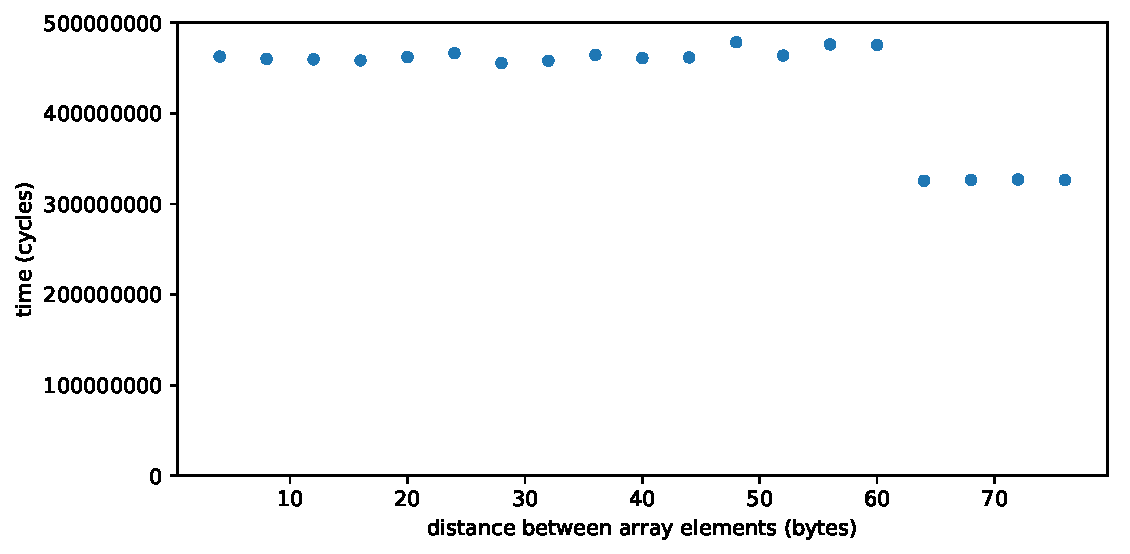
\includegraphics[width=\textwidth]{../sync/sum-up}
\end{frame}

\begin{frame}{false sharing}
\begin{itemize}
\item synchronizing to access two independent things
\vspace{.5cm}
\item two parts of same cache block
\item solution: separate them
\end{itemize}
\end{frame}

\subsubsection{exercise}
\begin{frame}[fragile,label=falseSharingEx1]{exercise (1)}
\begin{lstlisting}[
    language=C++,basicstyle=\tt\fontsize{8}{9}\selectfont,
    moredelim={**[is][\btHL<0|handout:0>]{@2}{2@}},
    moredelim={**[is][\btHL<0|handout:0>]{@3}{3@}},
    moredelim={**[is][\btHL<0|handout:0>]{@4}{4@}},
    escapeinside=QQ,
]
int @2values[1024]2@;
int @2results[2]2@;
void *sum_front(void *ignored_argument) {
    results[0] = 0;
    for (int i = @303@; i < @35123@; ++i)
        results[0] += values[i];
    return NULL;
}
void *sum_back(void *ignored_argument) {
    results[1] = 0;
    for (int i = @35123@; i < @310243@; ++i)
        results[1] += values[i];
    return NULL;
}
int sum_all() {
    pthread_t sum_front_thread, sum_back_thread;
    pthread_create(&sum_front_thread, NULL, sum_front, NULL);
    pthread_create(&sum_back_thread, NULL, sum_back, NULL);
    pthread_join(sum_front_thread, NULL);
    pthread_join(sum_back_thread, NULL);
    return @4results[0] + results[1]4@;
}
\end{lstlisting}
Where is false sharing likely to occur? How to fix?
\end{frame}

\begin{frame}[fragile,label=falseSharingEx2]{exercise (2)}
\begin{lstlisting}[
    language=C++,basicstyle=\tt\fontsize{8}{9}\selectfont,
    moredelim={**[is][\btHL<0|handout:0>]{@2}{2@}},
    moredelim={**[is][\btHL<0|handout:0>]{@3}{3@}},
    moredelim={**[is][\btHL<0|handout:0>]{@4}{4@}},
    escapeinside=QQ,
]
struct ThreadInfo { @2int *values;2@ int start; int end; int result };
void *sum_thread(void *argument) {
    ThreadInfo *@3my_info3@ = (ThreadInfo *) argument;Q\tikzmark{info}Q
    int sum = 0;
    for (int i = my_info->start; i < my_info->end; ++i) {
        my_info->result += my_info->values[i];
    }
    return NULL;

}
int sum_all(int *values) {
    ThreadInfo info[2]; pthread_t thread[2];
    for (int i = 0; i < 2; ++i) {
        @2info[i].values = values;2@ info[i].start = i*512; info[i].end = (i+1)*512;
        pthread_create(&threads[i], NULL, sum_thread, (void *) &info[i]);
    }
    for (int i = 0; i < 2; ++i)
        pthread_join(threads[i], NULL);
    return info[0].result + info[1].result;
}
\end{lstlisting}
Where is false sharing likely to occur?
\end{frame}


\section{cache coherency}
\section{preview: processor buses}
\usetikzlibrary{arrows.meta,matrix}

\begin{frame}{connecting CPUs and memory}
    \begin{itemize}
    \item multiple processors, common memory
    \item how do processors communicate with memory?
    \end{itemize}
\end{frame}

\begin{frame}{shared bus}
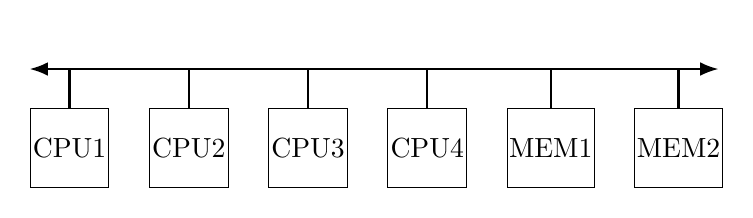
\begin{tikzpicture}
\matrix[
    matrix of nodes,
    nodes in empty cells,
    row 1/.style={nodes={minimum height=1cm,minimum width=1cm}},
    row 2/.style={nodes={draw,rectangle,minimum height=1cm,minimum width=1cm}},
    column sep=5mm,
] (net) {
      \& \& \& \& \&  \\
    CPU1 \& CPU2 \& CPU3 \& CPU4 \& MEM1 \& MEM2\\
};
\foreach \x in {1,2,3,4,5,6} {
    \draw[thick] (net-2-\x.north) -- (net-1-\x.center);
}
\draw[thick,Latex-Latex] (net-1-1.west) -- (net-1-6.east);
\end{tikzpicture}
\begin{itemize}
\item one possible design
    \begin{itemize}
    \item we'll revisit later when we talk about I/O
    \end{itemize}
\item \myemph{tagged} messages --- everyone gets everything, filters
\item contention if multiple communicators
    \begin{itemize}
    \item some hardware enforces only one at a time
    \end{itemize}
\end{itemize}
\end{frame}

\begin{frame}{shared buses and scaling}
    \begin{itemize}
    \item shared buses perform poorly with ``too many'' CPUs
    \item so, there are other designs
        \vspace{.5cm}
    \item we'll gloss over these for now
    \end{itemize}
\end{frame}

\begin{frame}{shared buses and caches}
    \begin{itemize}
    \item remember caches?
    \item memory is \myemph{pretty slow}
    \item each CPU wants to keep local copies of memory
        \vspace{.5cm}
    \item what happens when multiple CPUs cache same memory?
    \end{itemize}
\end{frame}


\subsection{problem setup / snooping}
\usetikzlibrary{arrows.meta,matrix,positioning,shapes.callouts}

\subsubsection{the cache coherency problem}

\begin{frame}[label=cacheShared]{the cache coherency problem}
\begin{tikzpicture}
\matrix[
    matrix of nodes,
    nodes in empty cells,
    row 1/.style={nodes={minimum height=1cm,minimum width=1cm}},
    row 2/.style={nodes={draw,rectangle,minimum height=1cm,minimum width=1cm}},
    column sep=2.75cm,
] (net) {
      \& \& \\
    CPU1 \& CPU2 \& MEM1 \\
};
\foreach \x in {1,2,3} {
    \draw[thick] (net-2-\x.north) -- (net-1-\x.center);
}
\draw[thick,Latex-Latex] (net-1-1.west) -- (net-1-3.east);
\tikzset{
    cache/.style={
        tight matrix,
        nodes={font=\small\ttfamily,text width=1.8cm},
        row 1/.append style={nodes={font=\small\bfseries}},
    },
}
\matrix[cache,anchor=north,label={[font=\small]south:CPU1's cache}] (cache1) at (net-2-1.south east){
    address \& value \\
    0xA300 \& \sout<2->{100}\only<2->{\myemph{101}} \\
    0xC400 \& 200 \\
    0xE500 \& 300 \\
};
\matrix[cache,anchor=north,label={[font=\small]south:CPU2's cache}] (cache2) at (net-2-2.south east){
    address \& value \\
    0x9300 \& 172 \\
    0xA300 \& 100 \\
    0xC500 \& 200 \\
};
\begin{visibleenv}<2->
\node[draw,thick,draw=blue,rectangle,anchor=north west] (writeTo) at ([yshift=-2cm]cache1.south west){
    \Large CPU1 writes 101 to 0xA300?
};
\node[my callout2=cache2-3-2,anchor=north] at ([yshift=-.5cm]cache2-3-2.south) {
    When does this change?
};
\node[my callout2=net-2-3.center,anchor=north] at ([yshift=-.5cm]net-2-3.center) {
    When does this change?
};
\end{visibleenv}
\end{tikzpicture}
\end{frame}



